In this section, we discuss the performance of \pred\ with respect to an increasing dimension for each task $m\in [M]$. Again note that the number of tasks $\Mpr \gg A \geq n$.
%
% Finally recall that when the horizon is small the weak demonstrator $\pi^w$ does not have sufficient samples for each action. This leads to a poor approximation of the greedy action. 
%
Through this experiment, we want to evaluate the performance of \pred\ and see how it exploits the underlying reward correlation when the horizon is small as well as for increasing dimensions.


\textbf{Baselines:} We again implement the same baselines discussed in \Cref{sec:short-horizon}. The baselines are \pred, \predt\ \dptg, \ad, \ts, and \linucb. 


\textbf{Outcomes:} We first discuss the main outcomes of our experimental results for increasing the horizon:

\begin{tcolorbox}
\customfinding \pred\ (\gt) outperforms \dptg, \ad\ with increasing dimension and has lower regret than \linucb\ for larger dimension.
\end{tcolorbox}

% \noindent
% \textbf{(1)} The \pred\ (\gt) learns to exploit the underlying latent structure and reward correlation between the different tasks even when $A \geq n$ but $\Mpr \gg A$.

% \textbf{(2)} The \pred\ (\gt) has lower regret than its weak demonstrator even when trained on $\Dtr\subseteq\Dpr$.

% \textbf{(3)} The \pred\ (\gt) has lower regret than \linucb\ for larger dimension.

% \begin{figure}[!hbt]
% \centering
% \begin{tabular}{ccc}
% \subfigure[Dimension $10$]{\hspace*{-1.5em}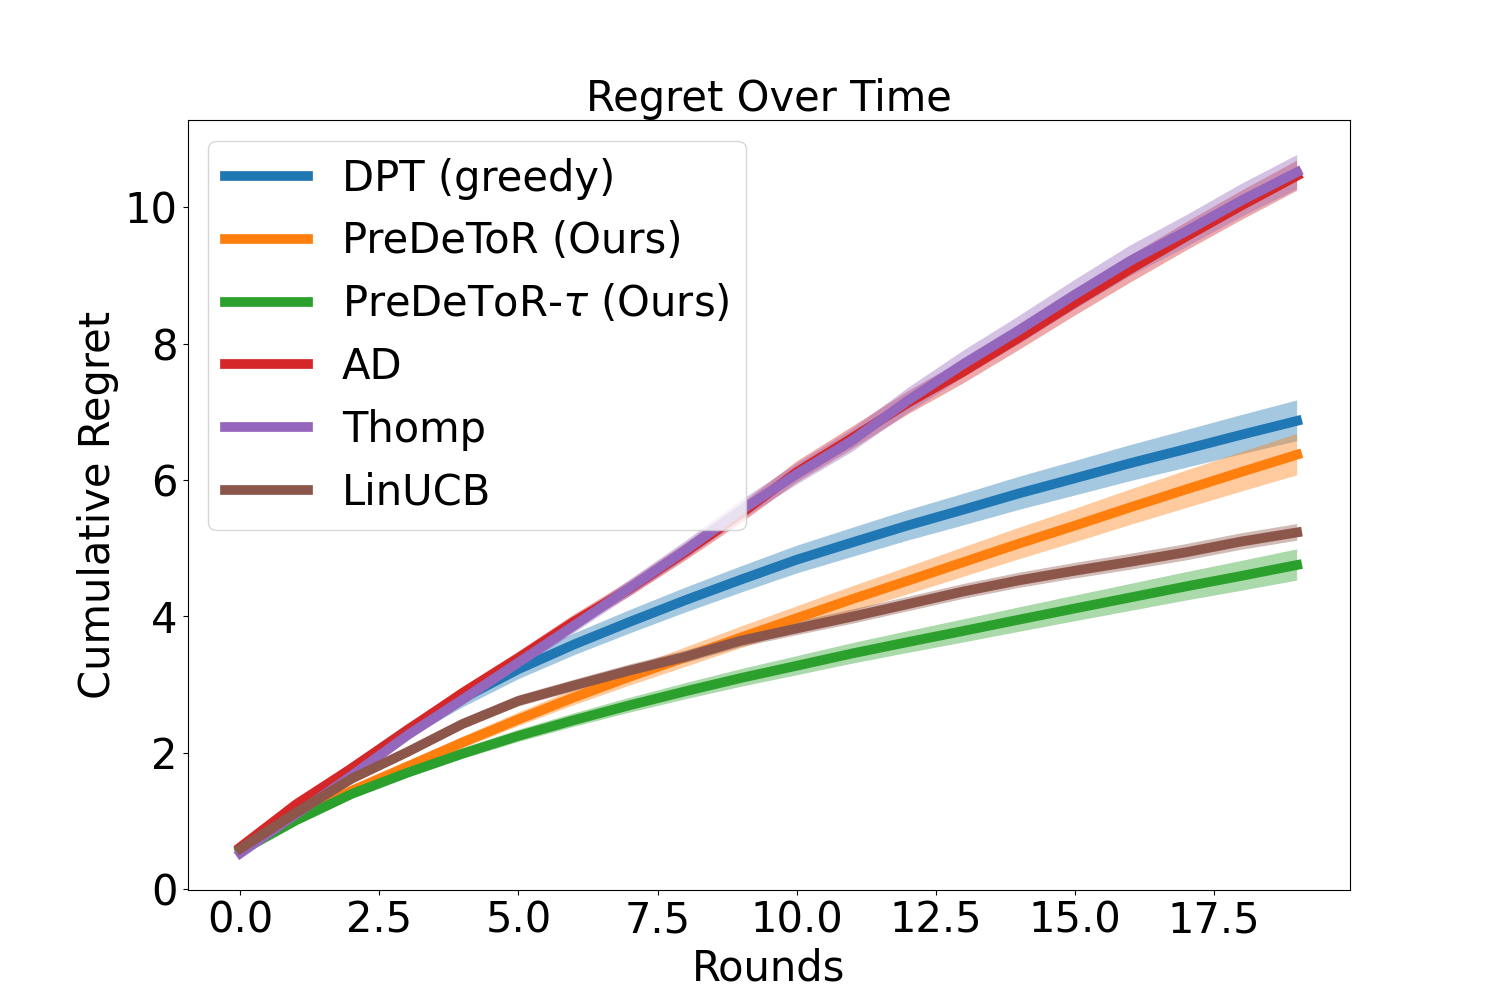
\includegraphics[scale = 0.13]{img/Neurips/dim/lin_d1_lr0.00015_do0_embd32_layer4_head4_envs160000_hists1_samples1_var0.3_cov0.0_H20_d20_lind10_seed1_testcov0.0_hor20.pkl.png}\label{fig:dim-10}} &
% %%%%%%%%%%
% \hspace*{-1.5em}\subfigure[Dimension $20$]{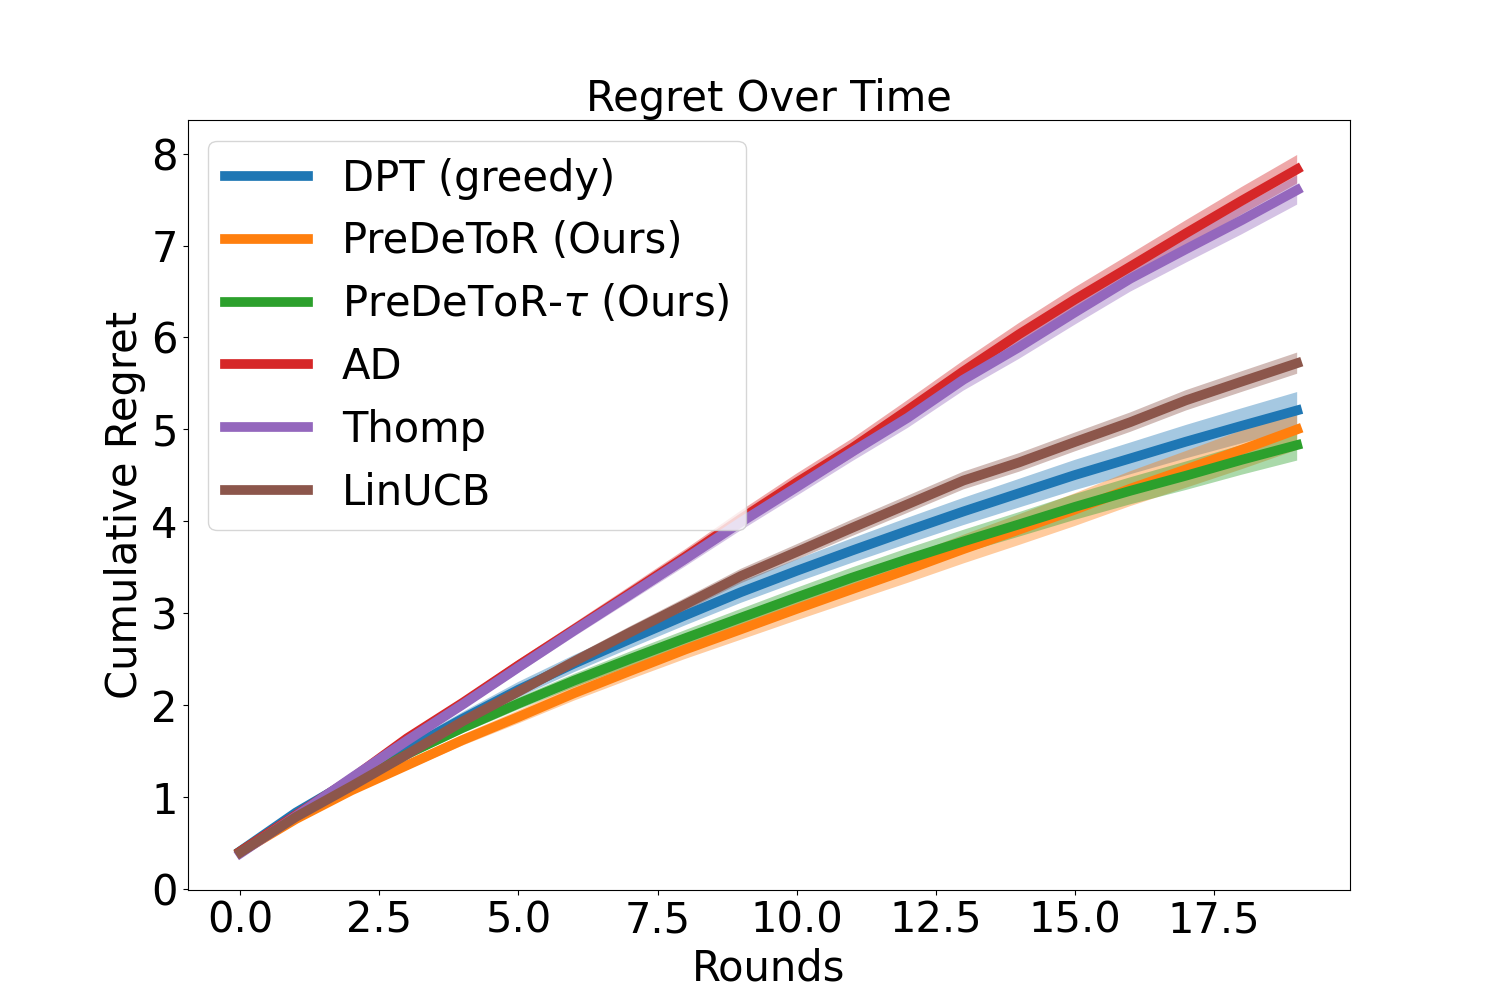
\includegraphics[scale = 0.13]{img/Neurips/dim/lin_d2_lr0.00015_do0_embd32_layer4_head4_envs160000_hists1_samples1_var0.3_cov0.0_H20_d20_lind20_seed1_testcov0.0_hor20.pkl.png} \label{fig:dim-20}} &
% %%%%%%%%%%%%%%%%%%%%%%%
% \subfigure[Dimension $30$]{\hspace*{-1.5em}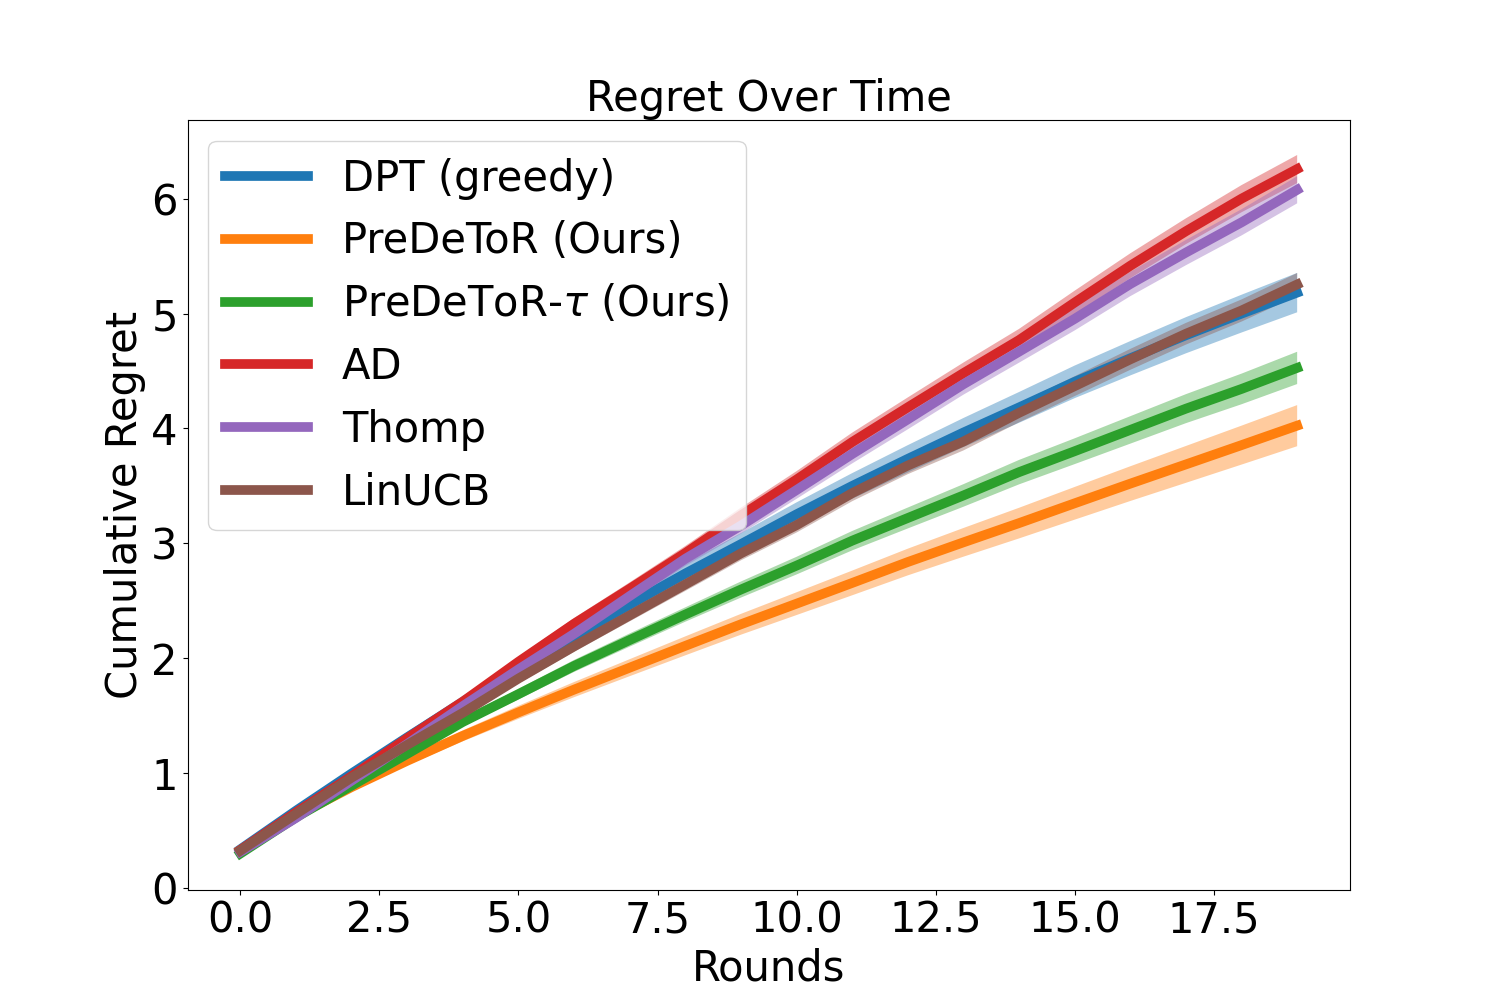
\includegraphics[scale = 0.13]{img/Neurips/dim/lin_d3_lr0.00015_do0_embd32_layer4_head4_envs160000_hists1_samples1_var0.3_cov0.0_H20_d20_lind30_seed1_testcov0.0_hor20.pkl.png}\label{fig:dim-30}} 
% \end{tabular}
% \begin{tabular}{cc}
% %%%%%%%%%%
% \hspace*{-1.5em}\subfigure[Dimension $40$]{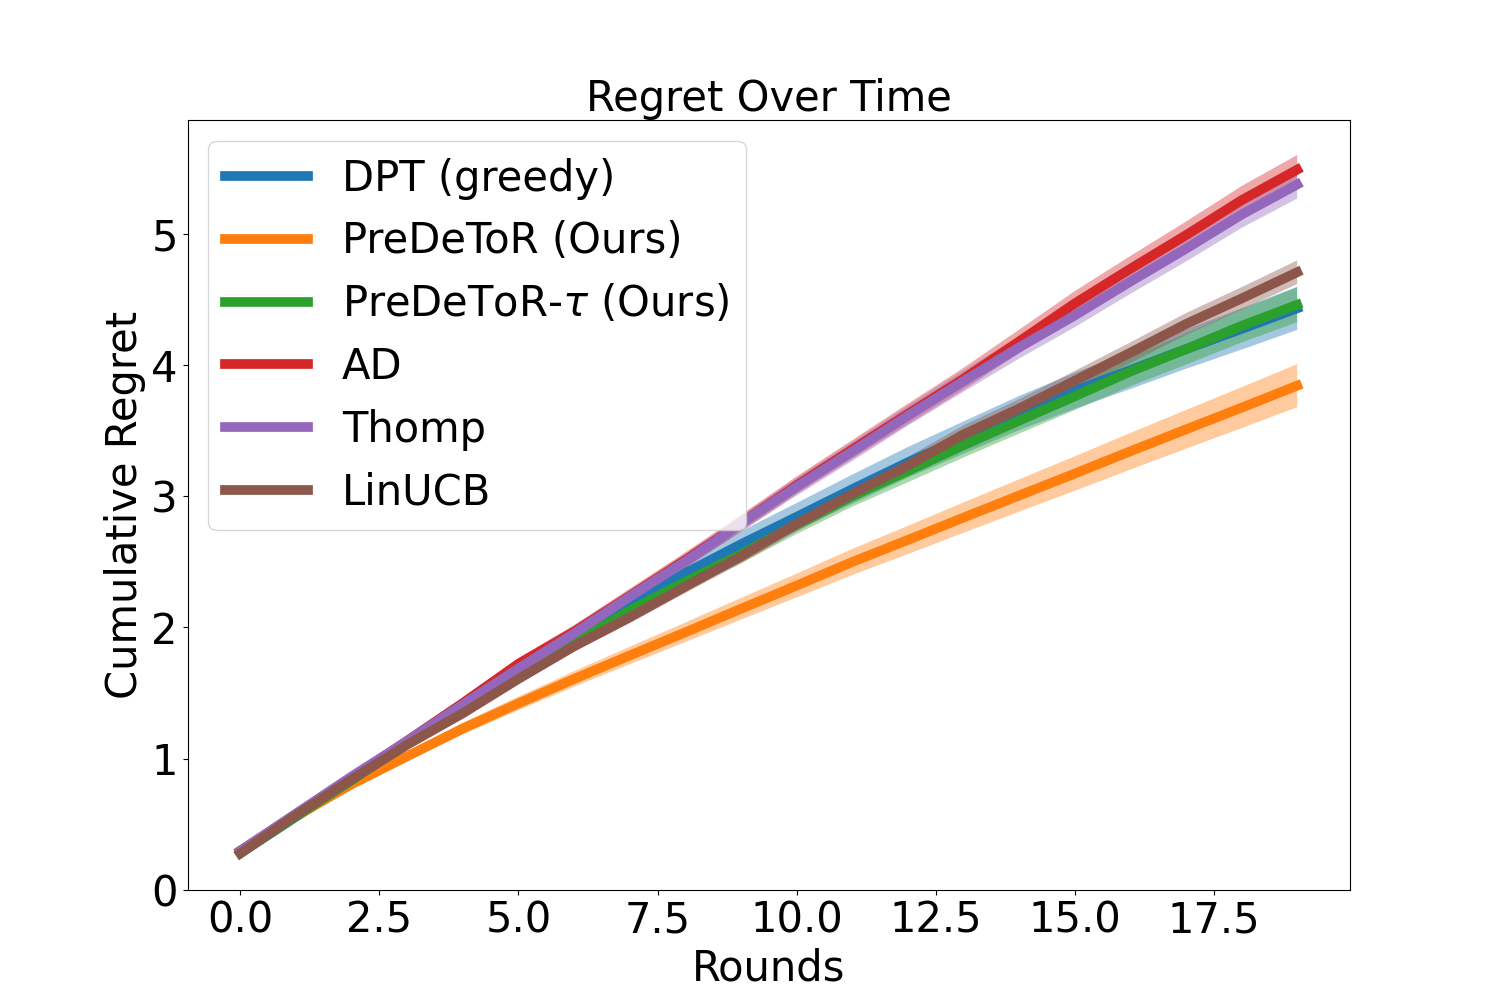
\includegraphics[scale = 0.13]{img/Neurips/dim/lin_d4_lr0.00015_do0_embd32_layer4_head4_envs160000_hists1_samples1_var0.3_cov0.0_H20_d20_lind40_seed1_testcov0.0_hor20.pkl.png} \label{fig:dim-40}} &
% %%%%%%%%%%%%%%%%%%%%%%%%%%%%%%%
% \hspace*{-1.5em}\subfigure[Increasing Dimension]{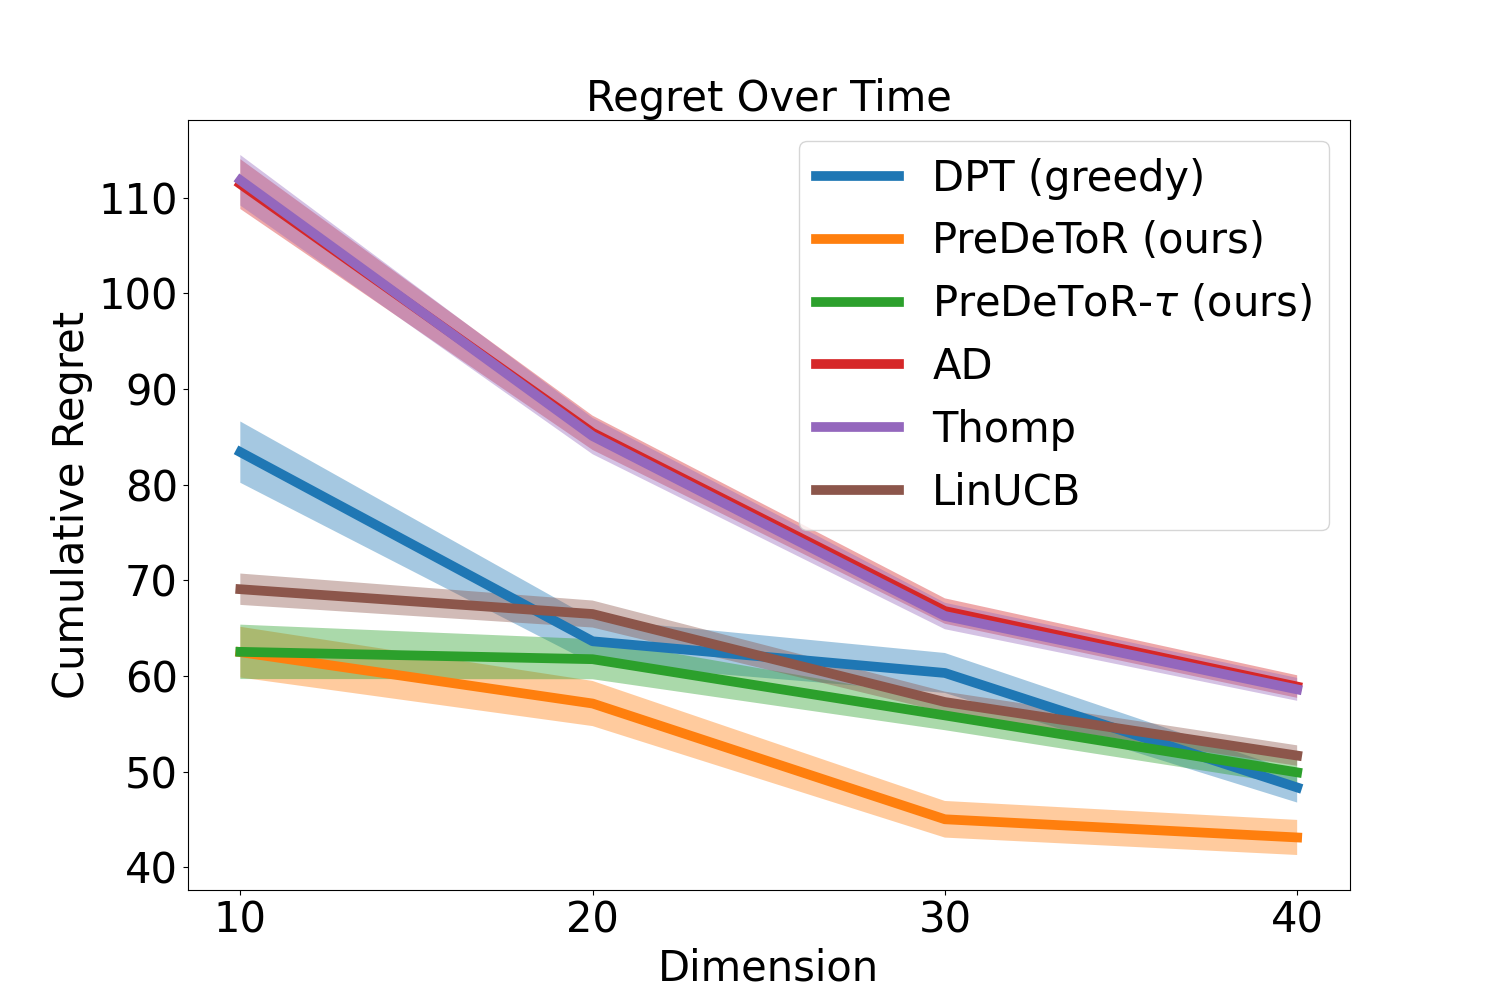
\includegraphics[scale = 0.13]{img/Neurips/dim/dim_fig.png} \label{fig:dim-inc}}
% \end{tabular}
% \vspace*{-1em}
% \caption{Experiment with increasing dimension. The y-axis shows the cumulative regret.}
% \label{fig:expt-dimension}
% \vspace{-0.7em}
% \end{figure}

\begin{figure}[!hbt]
\centering
\begin{subfigure}[b]{0.32\textwidth}
   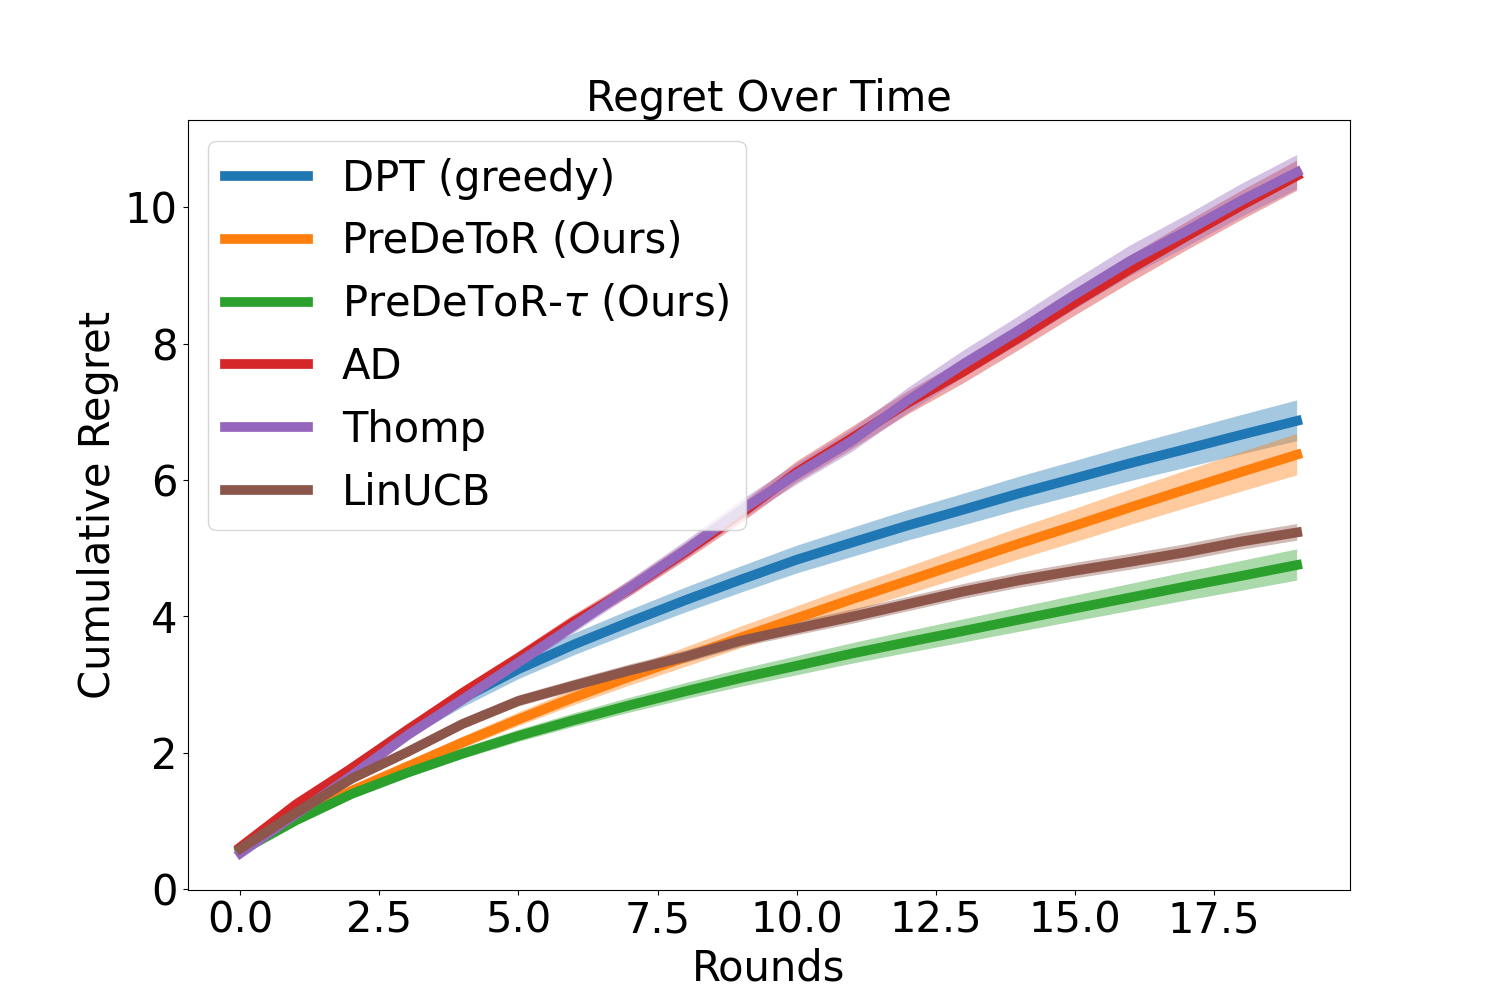
\includegraphics[scale=0.13]{img/Neurips/dim/lin_d1_lr0.00015_do0_embd32_layer4_head4_envs160000_hists1_samples1_var0.3_cov0.0_H20_d20_lind10_seed1_testcov0.0_hor20.pkl.png}
   \caption{Dimension $10$}
   \label{fig:dim-10}
\end{subfigure}%
\begin{subfigure}[b]{0.32\textwidth}
   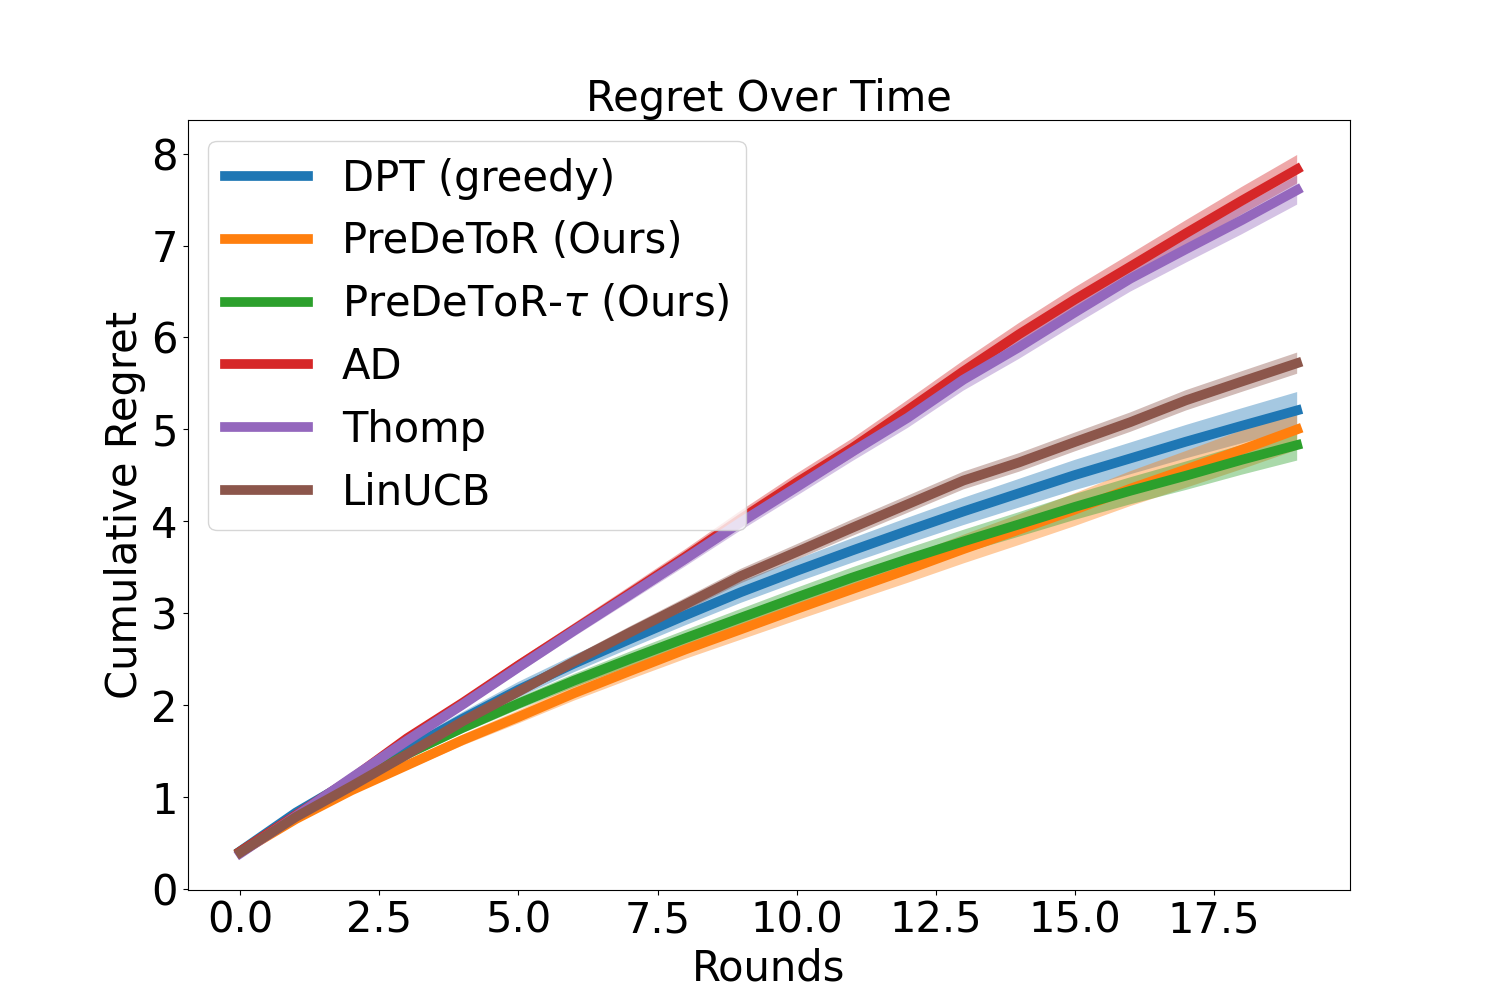
\includegraphics[scale=0.13]{img/Neurips/dim/lin_d2_lr0.00015_do0_embd32_layer4_head4_envs160000_hists1_samples1_var0.3_cov0.0_H20_d20_lind20_seed1_testcov0.0_hor20.pkl.png}
   \caption{Dimension $20$}
   \label{fig:dim-20}
\end{subfigure}%
\begin{subfigure}[b]{0.32\textwidth}
   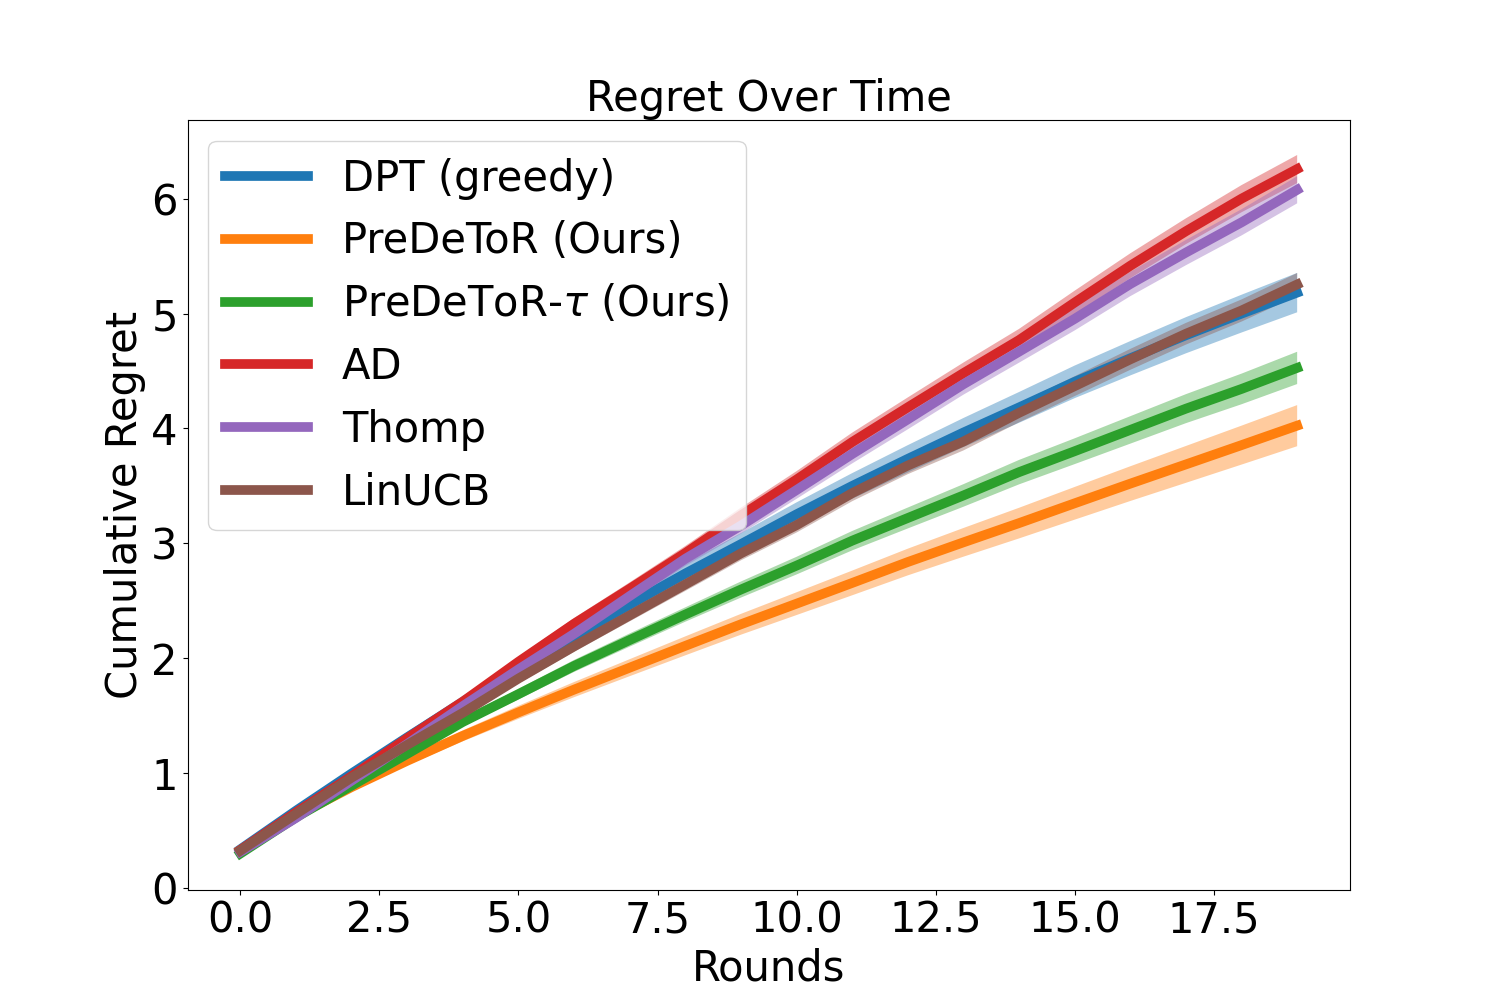
\includegraphics[scale=0.13]{img/Neurips/dim/lin_d3_lr0.00015_do0_embd32_layer4_head4_envs160000_hists1_samples1_var0.3_cov0.0_H20_d20_lind30_seed1_testcov0.0_hor20.pkl.png}
   \caption{Dimension $30$}
   \label{fig:dim-30}
\end{subfigure}

\begin{subfigure}[b]{0.48\textwidth}
   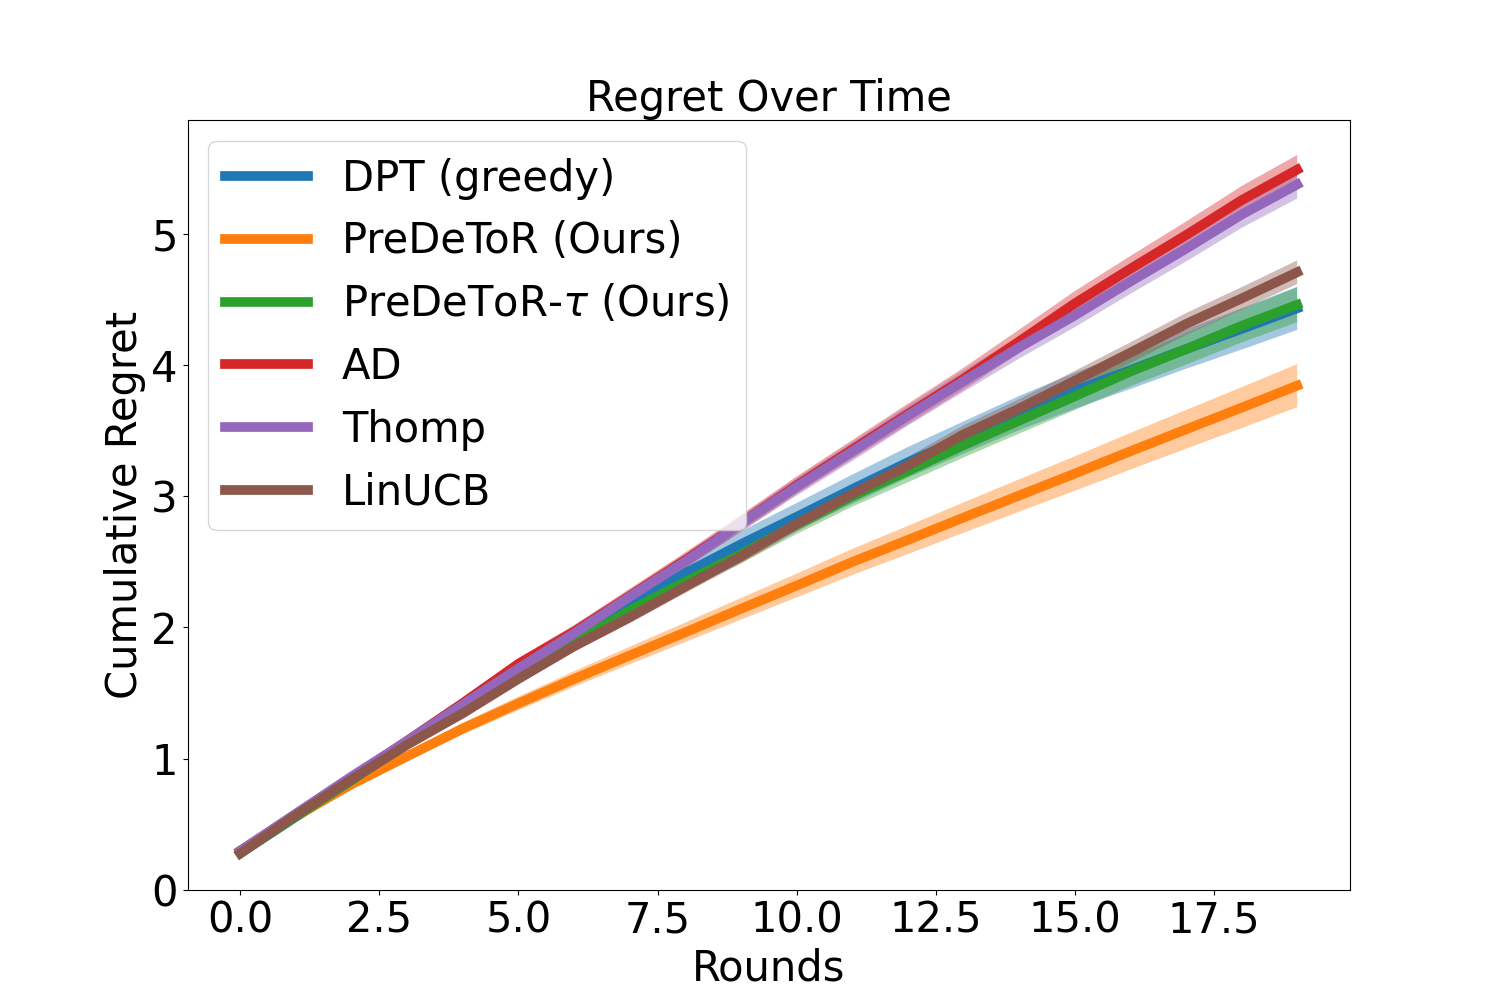
\includegraphics[scale=0.13]{img/Neurips/dim/lin_d4_lr0.00015_do0_embd32_layer4_head4_envs160000_hists1_samples1_var0.3_cov0.0_H20_d20_lind40_seed1_testcov0.0_hor20.pkl.png}
   \caption{Dimension $40$}
   \label{fig:dim-40}
\end{subfigure}%
\begin{subfigure}[b]{0.48\textwidth}
   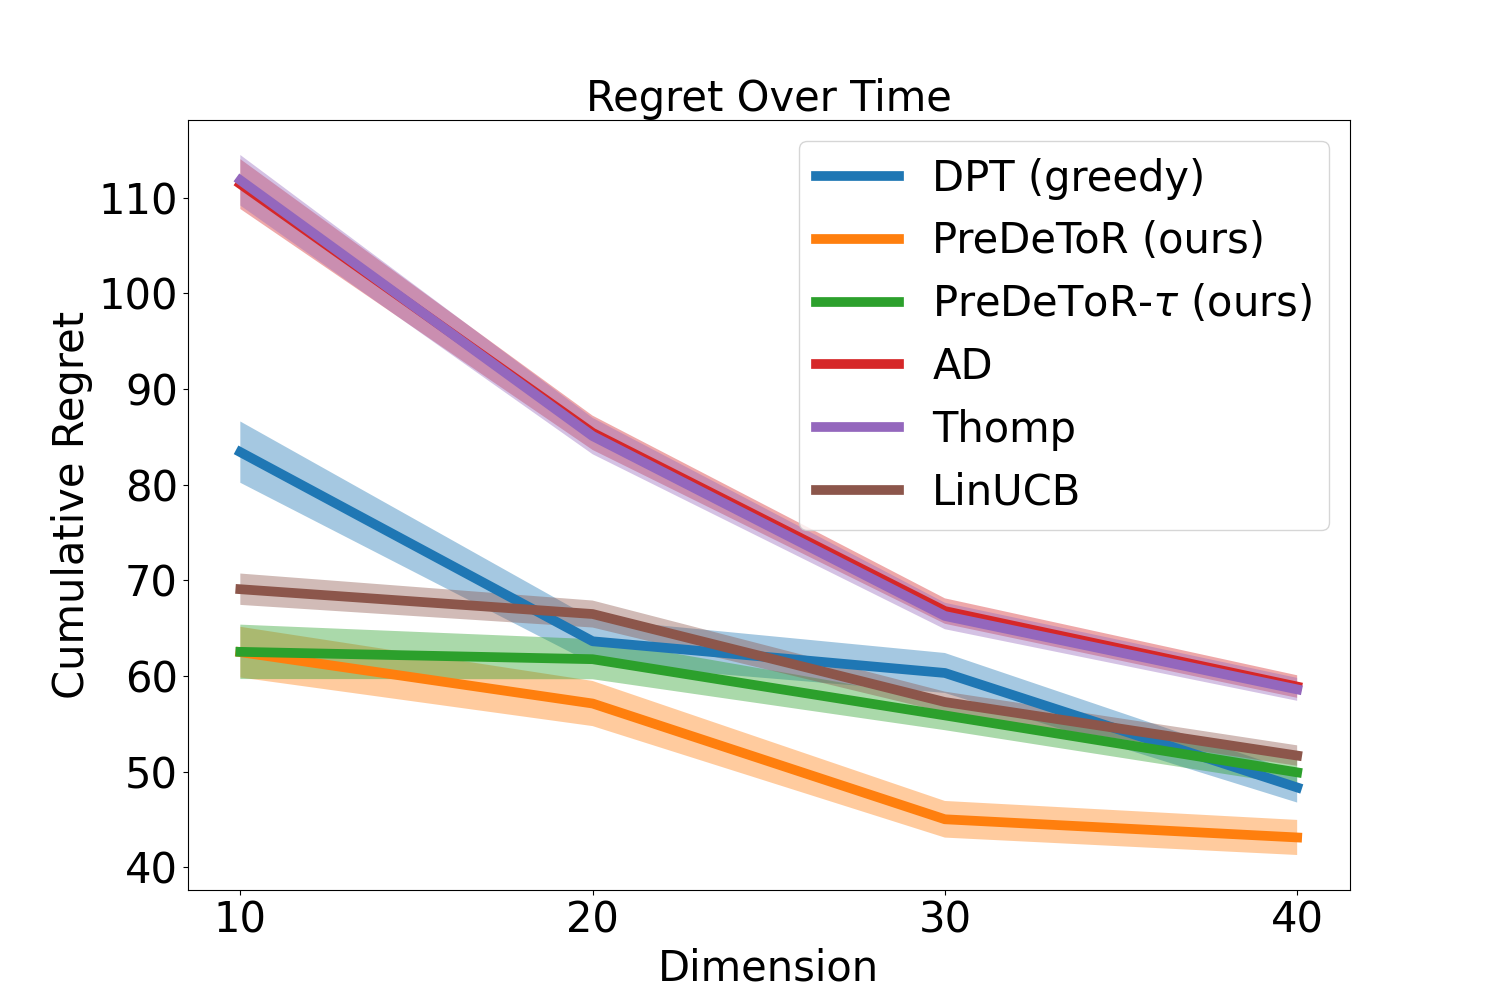
\includegraphics[scale=0.13]{img/Neurips/dim/dim_fig.png}
   \caption{Increasing Dimension}
   \label{fig:dim-inc}
\end{subfigure}
\vspace*{-1em}
\caption{Experiment with increasing dimension. The y-axis shows the cumulative regret.}
\label{fig:expt-dimension}
\vspace{-0.7em}
\end{figure}


\textbf{Experimental Result:} We observe these outcomes in \Cref{fig:expt-horizon}. In \Cref{fig:expt-horizon} we show the linear bandit setting for horizon $n=20$, $\Mpr =  160000$, $\Mts = 200$, $A=20$, and $d=\{10, 20, 30, 40\}$. 
%
%
Again, the demonstrator $\pi^w$ is the \ts\ algorithm. We observe that \pred\ (\gt) has lower cumulative regret than \dptg, \ad. Note that for any task $m$ for the horizon $20$ the \ts\ will be able to sample all the actions at most once.
% Moreover \pred\ matches the performance of \linucb. 
%
Observe from \Cref{fig:dim-10}, \ref{fig:dim-20}, \ref{fig:dim-30}, and \ref{fig:dim-40} that \pred\ (\gt) is closer to \linucb\ and has lower regret than \ts\ which also shows that \pred\ (\gt) is exploiting the latent linear structure of the underlying tasks.
%
In \Cref{fig:dim-inc} we plot the regret of all the baselines with respect to the increasing dimension. Again we see that \pred\ (\gt) has lower regret than \dptg, \ad\ and \ts. Observe that with  increasing dimension \pred\ is able to outperform \linucb. This shows that the \pred\ (\gt) is able to exploit reward correlation across tasks for varying dimensions.